%! Author = Juniell
%! Date = 10.05.2021

% Preamble
\documentclass[a4paper, 14pt]{extarticle}

% Packages
\usepackage[T2A]{fontenc}
\usepackage{natbib}
\usepackage{graphicx}
\usepackage[english, russian]{babel}
\usepackage{fontspec}
\usepackage{amsmath}
\usepackage{amsfonts}
\usepackage{amssymb}
\usepackage{amsthm}
\usepackage{mathtools}
\usepackage{mathrsfs}
\usepackage{fullpage}
\usepackage{ulem}
\usepackage{setspace}
\usepackage{listings}
\usepackage{indentfirst}
\usepackage[left=2cm,right=1.5cm,top=2cm,bottom=2cm]{geometry}
\usepackage{xcolor}
\usepackage{float}
\usepackage{csquotes}
\usepackage{hyperref}
\usepackage{graphics}

\definecolor{urlcolor}{HTML}{0000FF} % цвет ссылок
\definecolor{linkcolor}{HTML}{000000} % цвет гиперссылок
\hypersetup{pdfstartview=FitH, linkcolor=linkcolor, urlcolor=urlcolor, colorlinks=true}

\setmainfont{Times New Roman}
\setlength{\parindent}{5ex}
\setlength{\parskip}{1em}
\renewcommand{\baselinestretch}{1}

\graphicspath{{resources/Images}}

\definecolor{buzzlightyear}{HTML}{8757A5}
\definecolor{grass}{HTML}{738D06}
\definecolor{literal}{HTML}{F18A2B}
\definecolor{commentcolor}{HTML}{8E908B}

\lstdefinestyle{habrstyle}{
    backgroundcolor=\color{white},
    commentstyle=\color{commentcolor},
    keywordstyle=\bfseries\color{buzzlightyear},
    numberstyle=\tiny\color{commentcolor},
    stringstyle=\color{grass},
    basicstyle=\ttfamily\footnotesize,
    breakatwhitespace=false,
    breaklines=true,
    captionpos=b,
    keepspaces=true,
    numbers=left,
    numbersep=5pt,
    showspaces=false,
    showstringspaces=false,
    showtabs=false,
    tabsize=4,
    language=Python
}

\lstset{style=habrstyle}


% Document
\begin{document}
% Титульный лист
    \begin{center}
        \begin{center}
            \hfill \break
            \normalsize{Санкт-Петербургский государственный политехнический}\\
            \normalsize{университет Петра Великого}\\
            \hfill \break
            \normalsize{\textbf{Высшая школа интеллектуальных систем и}}\\
            \normalsize{\textbf{суперкомпьютерных технологий}}\\
            \hfill \break
            \hfill \break
            \hfill \break
            \hfill \break
            \hfill \break
            \normalsize{Отчёт по лабораторной работе №7}\\
            \normalsize{Дисциплина: Телекоммуникационные технологии}\\
            \normalsize{Тема: Дискретное преобразование Фурье}\\
        \end{center}
        \hfill \break
        \hfill \break
        \hfill \break
        \hfill \break
        \hfill \break
        \hfill \break
        \hfill \break
        \hfill \break
        \hfill \break
        \hfill \break
        \begin{tabbing}
            Выполнил студент гр. 3530901/80201 \`В.А. Пучкина\\
            \\
            Преподаватель: \`Н.В. Богач\\
        \end{tabbing}
        \hfill \break
        \hfill \break
        \hfill \break
        \hfill \break
        \begin{center}
            Санкт-Петербург\\
            2021
        \end{center}
        \thispagestyle{empty}
    \end{center}

% Оглавление
    \newpage
    \tableofcontents

% Список иллюстраций
    \newpage
    \listoffigures

% Список листингов
    \newpage
    \lstlistoflistings

% ---------------------------------------------- Упражнение 7.1 ----------------------------------------------
    \newpage
    \section{Упражнение 7.1}
    \label{sec:task1}

    В этом упражнении необходимо изучить примеры в файле \texttt{chap07.ipynb}.

    \begin{figure}[h]
        \centering
        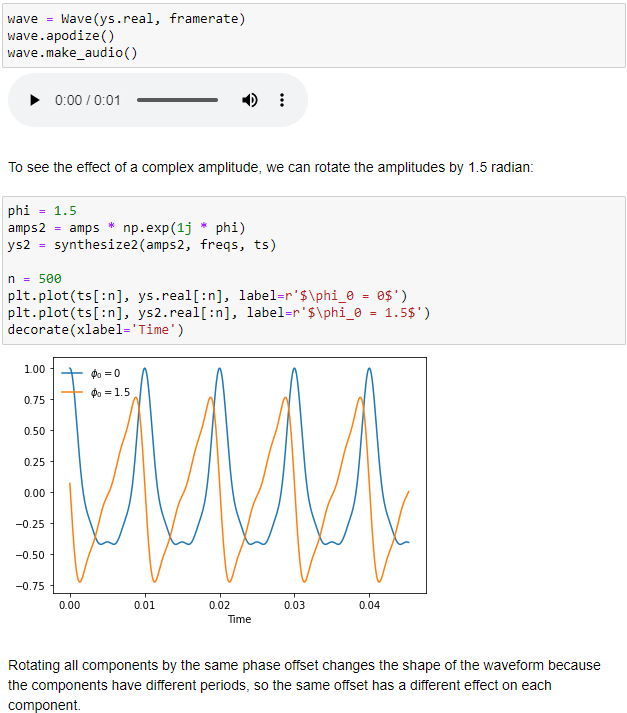
\includegraphics[width=0.8\linewidth]{resources/Images/task1_check}
        \caption{Изучение примеров.}
        \label{fig:task1_test_analyze1}
    \end{figure}

    Все примеры были запущены и изучены.

    \newpage

% ---------------------------------------------- Упражнение 7.2 ----------------------------------------------
    \section{Упражнение 7.2}
    \label{sec:task2}

    В данном упражнении необходимо реализовать быстрое преобразование Фурье (БПФ). Этот алгоритм позволяет ускорить
    преобразование Фурье с $N^2$ до $N log N$. Алгоритм выглядит следующим образом:

    \begin{enumerate}
        \item Дан массив сигнала $y$. Разделим его на чётные элементы $e$ и нечётные элементы $o$.
        \item Вычислим ДПФ $e$ и $o$, делая рекурсивные вызовы.
        \item Вычислим ДПФ($y$) для каждого значения $n$, используя лемму Дэниелсона-Ланцоша.
    \end{enumerate}
    В простейшем случае эту рекурсию надо продолжать, пока длина $y$ не дойдёт до 1. Тогда ДПФ($y$) = $y$.
    А если длина $y$ достаточно мала, можно вычислить его ДПФ перемножением матриц, используя заранее вычисленные матрицы.

    Итак, сначала нам потребуется определить функции \texttt{synthesis\_matrix} и \texttt{dft}, которые были использованы
    в примерах из \S\,\ref{sec:task1}.

    \begin{lstlisting}[caption= Функция \texttt{synthesis\_matrix}., label={lst:task2_fun_synthesis_matrix}]
PI2 = numpy.pi * 2

def synthesis_matrix(N):
    ts = numpy.arange(N) / N
    freqs = numpy.arange(N)
    args = numpy.outer(ts, freqs)
    M = numpy.exp(1j * PI2 * args)
    return M    \end{lstlisting}

    \begin{lstlisting}[caption= Функция \texttt{dft}., label={lst:task2_fun_dft}]
def dft(ys):
    N = len(ys)
    M = synthesis_matrix(N)
    amps = M.conj().transpose().dot(ys)
    return amps     \end{lstlisting}

    Теперь возьмём небольшой сигнал и вычислим его ДПФ с помощью функции \texttt{numpy.fft.fft}.

    \begin{lstlisting}[caption= Вычисление ДПФ с помощью \texttt{numpy.fft.fft}., label={lst:task2_dft_numpy}]
ys = [-0.2, 0.6, 0., -0.5]
hs = numpy.fft.fft(ys)
print(hs)   \end{lstlisting}

    \begin{lstlisting}[numbers=none, caption= Результаты для \texttt{numpy.fft.fft}., label={lst:task2_dft_numpy_res}]
[-0.1+0.j  -0.2-1.1j -0.3+0.j  -0.2+1.1j]   \end{lstlisting}

    А теперь сравним эти результаты с результатами, которые получатся при использовании функции \texttt{dft}
    (Листинг.\ref{lst:task2_fun_dft}).

    \begin{lstlisting}[caption= сравнение результатов функций \texttt{dft} и \texttt{numpy.fft.fft}., label={lst:task2_dft}]
ys = [-0.2, 0.6, 0., -0.5]
hs = numpy.fft.fft(ys)
print(hs)   \end{lstlisting}

    \begin{lstlisting}[numbers=none, caption= Результаты сравнения., label={lst:task2_dft_res}]
[-0.1+0.00000000e+00j -0.2-1.10000000e+00j -0.3+1.10218212e-16j -0.2+1.10000000e+00j]

6.230083922242757e-16   \end{lstlisting}

    Как видно из результатов сравнения, различия минимальны. А потому мы можем использовать \texttt{dft} в качестве
    <<основы>> для реализации БПФ.

    Теперь приступим к реализации алгоритма. Начнём с функции, разбивающей входной массив на чётные и нечётные элементы
    и использующей функцию \texttt{numpy.fft.fft} для вычисления ДПФ полученных половин вместо использования рекурсивного вызова.

    \begin{lstlisting}[caption= Функция \texttt{fft\_norec}., label={lst:task2_fun_fft_norec}]
def fft_norec(ys):
    N = len(ys)
    He = numpy.fft.fft(ys[::2])
    Ho = numpy.fft.fft(ys[1::2])

    ns = numpy.arange(N)
    W = numpy.exp(-1j * PI2 * ns / N)

    return numpy.tile(He, 2) + W * numpy.tile(Ho, 2)    \end{lstlisting}

    Вычислим БПФ с помощью этой функции и сравним полученный результат с другой реализацией.

    \begin{lstlisting}[caption= Сравнение результатов функциий \texttt{fft\_norec} и \texttt{numpy.fft.fft}., label={lst:task2_compare_norec}]
hs3 = fft_norec(ys)
print(hs3)
numpy.sum(numpy.abs(hs - hs3))  \end{lstlisting}

    \begin{lstlisting}[numbers=none, caption= Результаты сравнения., label={lst:task2_dft_res}]
[-0.1+0.0000000e+00j -0.2-1.1000000e+00j -0.3-1.2246468e-17j -0.2+1.1000000e+00j]

2.620466485321338e-16   \end{lstlisting}

    Как мы видим, разница всё ещё мала, что означает, что наша функция работает корректно.

    Теперь заменим нерекурсивные \texttt{numpy.fft.fft} на рекурсивные вызовы и добавим базовый случай.

    \begin{lstlisting}[caption= Функция \texttt{fft} с рекурсивными вызовами., label={lst:task2_fun_fft}]
def fft(ys):
    N = len(ys)
    if N == 1:
        return ys

    He = fft(ys[::2])
    Ho = fft(ys[1::2])

    ns = numpy.arange(N)
    W = numpy.exp(-1j * PI2 * ns / N)
    return numpy.tile(He, 2) + W * numpy.tile(Ho, 2)    \end{lstlisting}

    Сравним результаты функции \texttt{fft} с результатами другой реализации.

    \begin{lstlisting}[caption= Сравнение результатов функций \texttt{fft} и \texttt{numpy.fft.fft}., label={lst:task2_compare_fft}]
hs4 = fft(ys)
print(hs4)
numpy.sum(numpy.abs(hs - hs4))  \end{lstlisting}

    \begin{lstlisting}[numbers=none, caption= Результаты сравнения., label={lst:task2_fft_res}]
[-0.1+0.0000000e+00j -0.2-1.1000000e+00j -0.3-1.2246468e-17j -0.2+1.1000000e+00j]

4.0082452661027834e-16  \end{lstlisting}

    Как мы видим, полученная разница минимальна, а потому можно сказать, что написанная нами функция \texttt{fft}
    работает корректно. Более того, при такой реализации время выполнения составляет $N log N$ (вместо $N^2$).
    Однако и требуемое пространство пропорционально $N log N$. Кроме того, при такой реализации приходится тратить время
    на создание и копирование массивов.

    В ходе выполнения данного упражнения был реализован алгоритм БПФ, время выполнения которого составляет $N log N$
    (вместо $N^2$). Функция была протестирована сравнением её результатов с результатами \texttt{numpy.fft.fft}.
    Разница мала, а потому был сделан вывод, что составленная функция работает корректно. Также были разобраны
    достоинства (быстрое выполнение) и недостатки (требуется пространство и время для работы с массивами) такой реализации.

    \newpage

% ---------------------------------------------- Выводы ----------------------------------------------
    \section{Выводы}
    \label{sec:conclusions}

    В ходе выполнения данной лабораторной работы были изучены дискретное преобразование Фурье (ДПФ) и быстрое
    преобразование Фурье (БПФ). Кроме того, была написана функция, реализующая алгоритм БПФ. Она была протестирована, и
    был сделан вывод, что она работает корректно. При выборе используемой реализации преобразования Фурье стоит обращать
    внимание на длину массива сигнала. Если она мала, то будет достаточно использовать ДПФ (работает за $N^2$), если же длина большая, то
    стоит обратить внимание на БПФ (работает за $N log N$), чтобы уменьшить время вычисления. Однако при использовании
    конкретно этой реализации из \S\,\ref{sec:task2} важно помнить, что её требуемое пространство также пропорционально
    $N log N$.

\end{document}